
Due to space restrictions, we cannot include all the metrics of the training data. The complete training plots logs of our training are available on our GitLab repository. To illustrate the results of our first round of training, see Figures \ref{fig:07_vsi_sample_training_logs_unbalanced} and \ref{fig:07_vsi_sample_training_logs_pet_1000}. In the first figure, we can see that the optimal epoch to avoid overfitting is the fourth epoch, which coincidentally also maximizes the \fTwo{}, and in the second image, the first epoch is optimal, while it does not have the best \fTwo{}.


\begin{figure}[ht]
    \centering
    \subfigure[Training Loss]{
            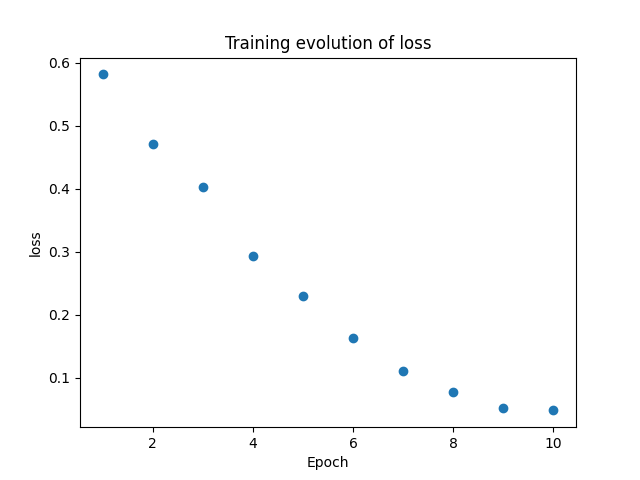
\includegraphics[width=0.3\textwidth]{Figures/07/sample_result/unbalanced_mbert_trafilatura_title_loss.png}
    }
    \hfill
    \subfigure[Development Loss]{
            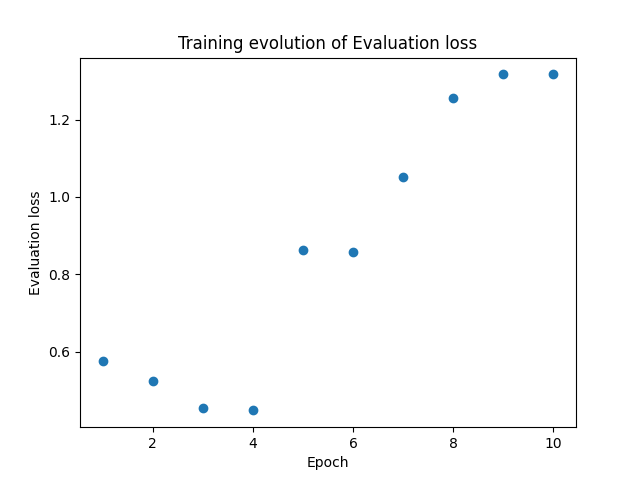
\includegraphics[width=0.3\textwidth]{Figures/07/sample_result/unbalanced_mbert_trafilatura_title_eval_loss.png}
    }
    \hfill
    \subfigure[Development \fTwo{}]{
            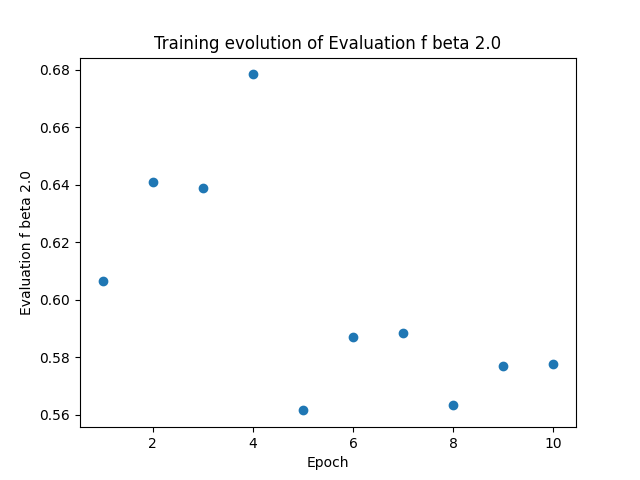
\includegraphics[width=0.3\textwidth]{Figures/07/sample_result/unbalanced_mbert_trafilatura_title_eval_f_beta_2.0.png}
    }
    \caption{\unbalanced{} - Losses and Development \fTwo{} evolution for \bertmultilingual{} on the \trafilaturaTitle{}}
    \label{fig:07_vsi_sample_training_logs_unbalanced}
\end{figure}


\begin{figure}[ht]
    \centering
    \subfigure[Training Loss]{
            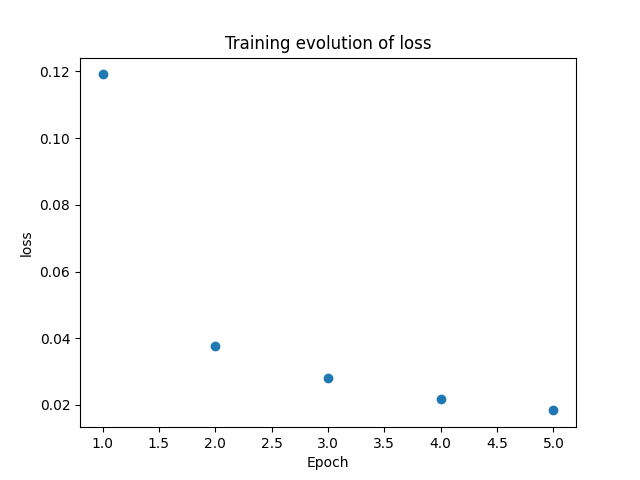
\includegraphics[width=0.3\textwidth]{Figures/07/sample_result/pet1000_roberta_trafilatura_title_loss.png}
    }
    \hfill
    \subfigure[Development Loss]{
            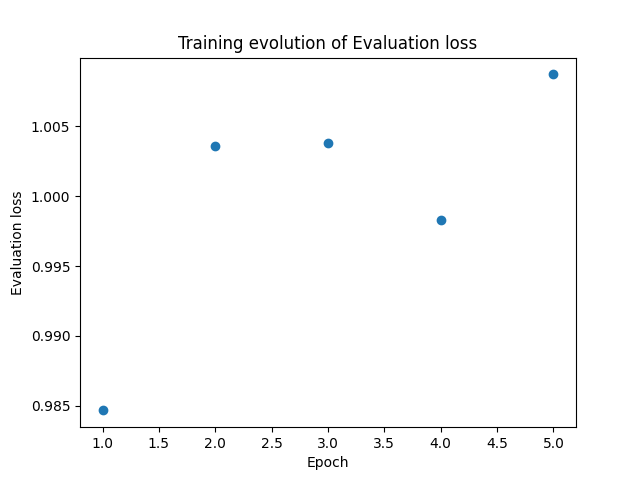
\includegraphics[width=0.3\textwidth]{Figures/07/sample_result/pet1000_roberta_trafilatura_title_eval_loss.png}
    }
    \hfill
    \subfigure[Development \fTwo{}]{
            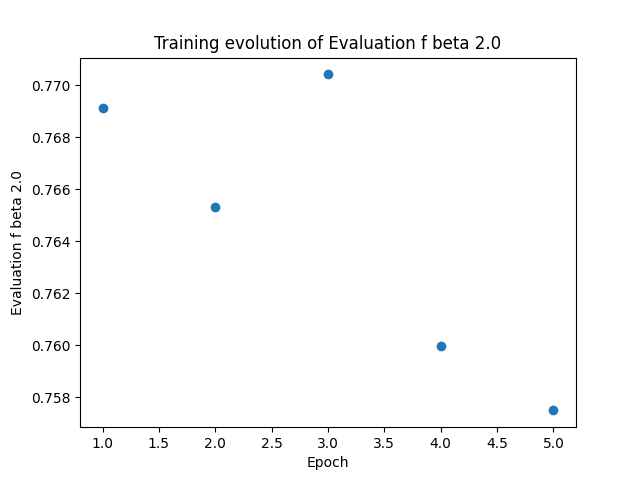
\includegraphics[width=0.3\textwidth]{Figures/07/sample_result/pet1000_roberta_trafilatura_title_eval_f_beta_2.0.png}
    }
    \caption{\petThousand{} - Losses and Development \fTwo{} evolution for \bertroberta{} on the \trafilaturaTitle{}}
    \label{fig:07_vsi_sample_training_logs_pet_1000}
\end{figure}


The optimal epochs for each training scenario can be found in \appendixname{} \ref{appendix05:vsi_optimal_epochs}. It is immediately clear that \unbalanced{} is the slowest method to reach the optimal epoch, as all the other methods have more than half of the optimal epochs be either 1 or 2. In fact, between the two \finetuning{} techniques, there is a huge gap in favor of \balanced{}, which, for most cases, takes only one epoch to reach the optimum. As for \gls{pet}, the five scenarios show very similar behavior, in general reaching the optimal epoch before the fourth epoch. This makes us think that, if there are differences in convergence speed, they must happen during the training of the \gls{pet} Ensembles. As all the Ensembles are trained for five epochs, this must be enough for them to get decent performance. Unfortunately, we did not log the evolution of the custom losses calculated during training the \gls{pet} Ensembles.


Using these results, we were able to proceed to the second training round, and train models up to the optimal epochs and evaluate their performance there. In \appendixname{} \ref{appendix05:vsi_metrics_optimal_epochs} one can find the metrics for the optimal classifiers for each training scenario, for each \gls{bert} model. By comparing the results for the Development \fTwo{}, it is immediately clear that \unbalanced{} has the worst performance of all the training methods\footnote{An \fTwo{} of 0\% means that the model defaulted to predict the majority class (negative)}. In fact, it is surpassed by \balanced{} in all cases but one\footnote{This particular case is \bertbase{} on the \trafilaturaTitle{}, with a difference of approximately 3\%}. 
Regarding \gls{pet}, there is a clear performance improvement as the number of documents per category increases. On one hand, the Development \fTwo{} for \petFifty{} is in general lower than for the other \gls{pet}s and only rarely compares to them. On the other hand, \petFiveHundred{} and \petThousand{} consistently achieve the best performance.

Given the high number of training scenarios ($336$), we may impose a high performance threshold, and only consider those classifiers with at least around 80\% Development \fTwo{}. There are 72 classifiers that satisfy this constraint, which is round one fifth of  all scenarios. These can be found summarized in Table \ref{appendix05:tab:f2_auc_top_pergorming_by_model}, where it can be seen that training with \gls{pet} almost always outperforms \finetuning{}\footnote{Except for \bertxlmroberta{} on the \trafilaturaFulltext{}}, and that \unbalanced{} never makes it to the list. Within the \gls{pet} setups, using \petFiveHundred{} and \petThousand{} guarantees performing over the threshold. 

The top \gls{bert} models by number of top classifiers are \bertxlmroberta{} (22), \bertmultilingual{} (16), and \bertbiolinkbert{} (16). This may be an indication that the multilingual aspect of our dataset is more relevant than its biomedical aspect for determining relevance. This is consistent with the observation that 4 top classifiers correspond to \bertscibert{}, and only 3 to \bertbase{}. \bertroberta{} falls somewhat in the middle, with 11 top classifiers, which may reflect that overall it is a more powerful model than \bertbase{} and \bertscibert{}, but being only trained for English limits it.


At the same time, we can notice that several of the top classifiers have alarmingly low Development \auc{}s, between 60\% and 80\% (Figure \ref{fig:07_vsi_sample_auc}). A low \auc{} means that these models have trouble distinguishing positives and negatives, while a high \fTwo{} means that they have a high recall compared to precision. Combining these observations, we can say that these models are obtaining a high \fTwo{} by almost defaulting to mark all documents as positive.



\begin{figure}[ht]
    \centering
    \subfigure[\bertbiolinkbert{} with \petFifty{} on the \trafilaturaTitle{}]{
            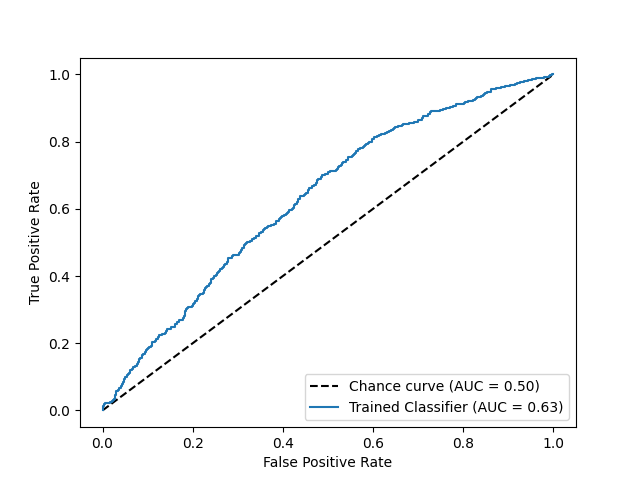
\includegraphics[width=0.3\textwidth]{Figures/07/sample_auc/biolinkbert_pet_50_trafilatura_title_dev_ROC_on_split.png}
    }
    \hfill
    \subfigure[\bertroberta{} with \petTwoHundred{} on the \trafilaturaFulltext{}]{
            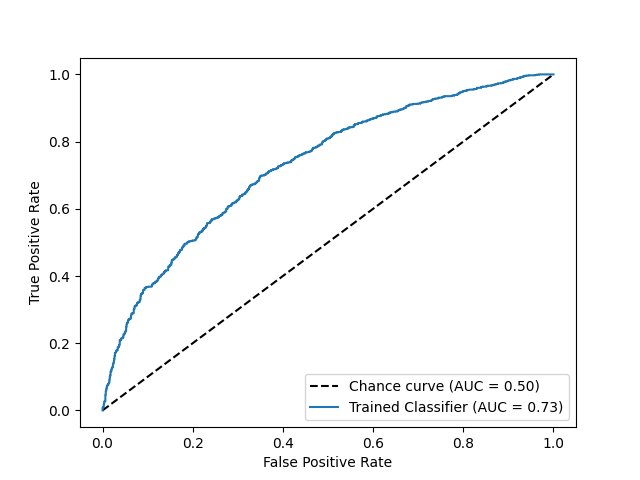
\includegraphics[width=0.3\textwidth]{Figures/07/sample_auc/roberta_pet_200_trafilatura_fulltext_dev_ROC_on_split.png}
    }
    \hfill
    \subfigure[\bertxlmroberta{} with \petThousand{} on the \trafilaturaFulltext{} ]{
            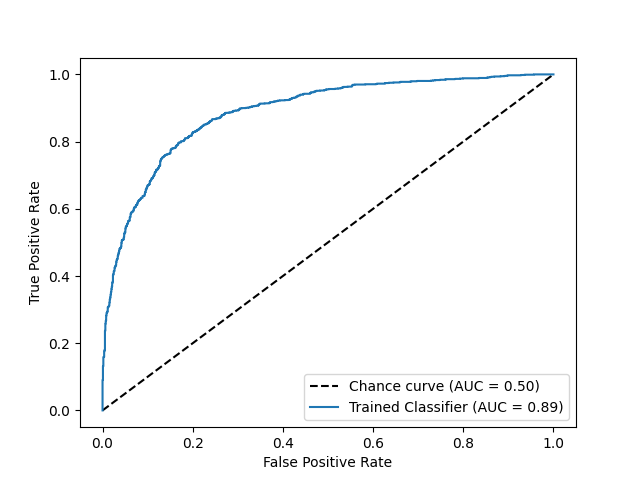
\includegraphics[width=0.3\textwidth]{Figures/07/sample_auc/xlmroberta_pet_1000_fulltext_dev_ROC_on_split.png}
    }
    \caption{Sample \auc{}s for some classifiers}
    \label{fig:07_vsi_sample_auc}
\end{figure}

As we prefer models that actually ``understand" what relevance means, instead of just flagging everything as a positive, we decide to impose a threshold of 80\% for the Development \fTwo{}. In this way, we obtain 49 scenarios, summarized in Table \ref{appendix05:tab:f2_auc_f1_top_pergorming_by_content_type}. It is notable that the \contentType{} with the most top classifiers is the \trafilaturaFulltext{}, obtaining 15 top classifiers over all the \gls{bert} models. This suggests that the \trafilaturaFulltext{}, being on average much longer than the other \contentType{}s, provides enough content so that the task can be well learned by any of the models.

At the same time, note that the \keyphrasesAbstractOnly{} do \textbf{not} make it to the list. As explained at the end of \headerName{} \ref{vsi_preprocessing}, this dataset is severely reduced during preprocessing, and thus, may not be left with enough content. Since we still have four top classifiers for the \trafilaturaAbstract{}, we decide to \textbf{discard} the \keyphrasesAbstractOnly{} as a \contentType{}.

To avoid classifiers that flag almost everything as a positive, we impose a 75\% threshold on the Development \fOne{}. In this way, we are left with 17 classifiers. Table \ref{appendix05:tab:metrics_for_best_classifiers} contains all the Development and Test metrics for these classifiers, highlighting the best metrics. Again, the \trafilaturaFulltext{} the most classifiers in this list (9), and we highlight the best three metrics. 

As one would expect, the Test metrics are lower than the Development metrics. However, it is immediately noticeable that, the \fOne{} and precision decrease considerable, going below 50\% in most cases. This may be explained by our focus on the \fTwo{}, which disfavors Precision and favors Recall. At the same time, the best Test Recalls are close to 80\% and above.

Note that the \keyphrasesFulltextOnly{} does not make it to the list. As before, this may be explained by the fact that taking only the sentences containing keywords really decreases the content of the dataset. At the same time, notice that the top metrics for the \keyphrasesAbstractOC{} and the \keyphrasesFulltextOC{} are always below the \trafilaturaAbstract{} and the \trafilaturaFulltext{}. These observations imply that leveraging the keywords in the content does \textbf{not} help improve performance, contrary to our hypothesis in \headerName{} \ref{vsi_leveraging_keywords}. Thus, we decide to not include these sources of content moving forward.

Taking the best performing classifiers (Table \ref{tab:07_best_classifiers}), we are left with the four original \contentType{}s and the classifiers we will use for our system. Note that all but one of the best classifiers are obtained with \petThousand{}. Also, all the best classifiers are obtained with the multilingual \gls{bert} models. This reinforces the idea that the multilingual aspect of our data is crucial for determining relevance, instead of the biomedical aspect.

\begin{table}[ht]
\resizebox{\textwidth}{!}{
\begin{tabular}{|l|c|c|ccc|c|}
\hline
\contentType{}       & \trafilaturaTitle{}    & \trafilaturaAbstract{}    & \trafilaturaFulltext{} & \trafilaturaFulltext{}           & \trafilaturaFulltext{}   & \translationTitle{} \\ 
Model           & \bertmultilingual{}                 & \bertxlmroberta{}           & \bertmultilingual{}                 & \bertxlmroberta{}           & \bertxlmroberta{}           & \bertmultilingual{}                 \\
Training Method & \petThousand{}              & \petThousand{}              & \petThousand{}              & \balanced{}   & \petThousand{}              & \petThousand{}              \\ \hline
Development \fTwo{}  & \mycoloredcell{0.8244310265} & \mycoloredcell{0.8233701782} & \mycoloredcell{0.8274771609} & \mycoloredcell{0.8361531612} & \mycoloredcell{0.8573388203} & \mycoloredcell{0.8286908078} \\
Development \auc{}       & \mycoloredcell{0.8345520661} & \mycoloredcell{0.8415276893} & \mycoloredcell{0.8882393048} & \mycoloredcell{0.9057368386} & \mycoloredcell{0.8884577866} & \mycoloredcell{0.8526575213} \\
Development \fOne{}  & \mycoloredcell{0.7755324959} & \mycoloredcell{0.7741251326} & \mycoloredcell{0.8152315015} & \mycoloredcell{0.8395172105} & \mycoloredcell{0.8159934721} & \mycoloredcell{0.7880794702} \\
Development Accuracy  & \mycoloredcell{0.7509090909} & \mycoloredcell{0.7491166078} & \mycoloredcell{0.8105590062} & \mycoloredcell{0.8405861456} & \mycoloredcell{0.7999112689} & \mycoloredcell{0.7692307692} \\
Development Precision & \mycoloredcell{0.7057654076} & \mycoloredcell{0.7039537126} & \mycoloredcell{0.7956081081} & \mycoloredcell{0.8451845185} & \mycoloredcell{0.7552870091} & \mycoloredcell{0.7285714286} \\
Development Recall    & \mycoloredcell{0.8606060606} & \mycoloredcell{0.8598351001} & \mycoloredcell{0.8358473824} & \mycoloredcell{0.8339253996} & \mycoloredcell{0.8873114463} & \mycoloredcell{0.8581730769} \\ \hline
Test \fTwo{}         & \mycoloredcell{0.6055995131} & \mycoloredcell{0.6056860321} & \mycoloredcell{0.6696935301} & \mycoloredcell{0.637195122}  & \mycoloredcell{0.6379132231} & \mycoloredcell{0.6380890052} \\
Test \auc{}        & \mycoloredcell{0.8249796338} & \mycoloredcell{0.8460210289} & \mycoloredcell{0.8961402345} & \mycoloredcell{0.8721908143} & \mycoloredcell{0.896623166}  & \mycoloredcell{0.8419944312} \\
Test Precision  & \mycoloredcell{0.2783216783} & \mycoloredcell{0.2873900293} & \mycoloredcell{0.5021276596} & \mycoloredcell{0.511002445}  & \mycoloredcell{0.4434470377} & \mycoloredcell{0.318627451}  \\
Test Recall     & \mycoloredcell{0.8577586207} & \mycoloredcell{0.8376068376} & \mycoloredcell{0.7923691216} & \mycoloredcell{0.8223801066} & \mycoloredcell{0.7249334516} & \mycoloredcell{0.8515283843} \\
Test \fOne{}         & \mycoloredcell{0.4202745512} & \mycoloredcell{0.4279475983} & \mycoloredcell{0.3543543544} & \mycoloredcell{0.3841911765} & \mycoloredcell{0.294047619}  & \mycoloredcell{0.4637336504} \\
Test Accuracy   & \mycoloredcell{0.6672727273} & \mycoloredcell{0.691401649}  & \mycoloredcell{0.8613138686} & \mycoloredcell{0.7627737226} & \mycoloredcell{0.901459854}  & \mycoloredcell{0.7289663462} \\ \hline
\end{tabular}
}
\caption{Best classifiers by \contentType{}}
\label{tab:07_best_classifiers}
\end{table}


Finally, we propose an explanation for the better performance of \gls{pet} over \finetuning{}. Our hypothesis is that, by using task descriptions, \gls{pet} helps the model get a better understanding of the task.
To explain this point, we borrow an example from the original \gls{pet} paper by \mytextcite{pet_paper}.

Consider the following three sentences, where the first two are labelled, and we are tasked to label the third one:

\begin{itemize}
    \item[1.] Category A: This \textit{was} the best \textit{pizza} I've ever had.
    \item[2.] Category B: You \textit{can} get better sushi for half the \textit{price}.
    \item[3.] Category ?: \textit{Pizza} \textit{was} average. Not worth the \textit{price}.
\end{itemize}
\vspace{4pt}
Just with this information, it is hard to assign a label: Is the task about pizza? Or is it about detecting verb tense (Past VS Present)? However, if we are told that the task is to find the sentences talking about pizza, we would immediately assign category A to the third sentence, and if the task is about prices, we would assign Category B.


For our task, consider the three following (artificial) sentences:

\begin{itemize}
    \item[1.] Relevant: Oriental Fruit fly (Bactrocera dorsalis) detected in a new location in Central Asia.
    \item[2.] Irrelevant: Check out the best decorative plants for your garden this summer, and beware of insects! 
    \item[3.] Category ?: What to do if you find fruit flies plaguing your field - Agriculture News Online. 
\end{itemize}
\vspace{4pt}



Our task being detection of document relevance for Plant Health Surveillance, we assign the third sentence to the Irrelevant category, however, this nuance may be lost to a language model, needing supplementary knowledge.

In fact, looking at Table \ref{tab:07_best_classifiers}, notice that the only time that  \finetuning{} produces one of the best classifiers, it is for the \trafilaturaFulltext{}. Additionally, along our discussion, we have seen that several of the top performing classifiers are trained on the \trafilaturaFulltext{}. These observations suggest that the \trafilaturaFulltext{}, being longer than all the other \contentType{}s (1102 tokens on average), has enough content so that any \gls{bert} model eventually picks up the task.
All the other \contentType{}s, being significantly shorter than the \trafilaturaFulltext{}, do not provide enough content for the models (on average, the \trafilaturaTitle{} has 11 tokens, the \trafilaturaAbstract{} has 50, and the \translationTitle{} has 12), and thus, the classifiers benefit from the additional knowledge provided by \gls{pet} patterns.
Also, notice that all the other best classifiers are trained using \petThousand{}. This means that, the more one shows the model examples of documents plus knowledge about the task, the better performance one gets. However, this performance gains eventually stale, as one can see that the gains from using \petFiveHundred{} to \petThousand{} are only a couple of points (Tables \ref{tab:07_f2_bert_base}-\ref{tab:07_f2_bert_xlmroberta}).
In conclusion, by using \gls{pet} and its patterns, we inject task-specific knowledge, guiding the model. 


\clearpage